%File: main.tex
%Based on formatting-instructions.tex, distributed as part of the aaai submission information.
\documentclass[letterpaper]{article}
\usepackage{aaai}
\usepackage{times}
\usepackage{helvet}
\usepackage{courier}
\frenchspacing

% Package and images path
\usepackage{graphicx}
\graphicspath{ {images/} }

\setlength{\pdfpagewidth}{8.5in}
\setlength{\pdfpageheight}{11in}
\pdfinfo{
/Title (Link Prediction in FanFiction Networks)
/Author (Alexander Hayes)}
\setcounter{secnumdepth}{0}

\begin{document}
% The file aaai.sty is the style file for AAAI Press
% proceedings, working notes, and technical reports.
%

\title{Link Prediction in FanFiction Networks}
\author{Alexander L. Hayes\\
The University of Texas at Dallas\\
alexander.hayes@utdallas.edu\\
}

\maketitle
\begin{abstract}
\begin{quote}
The author performs link prediction on metadata and social network data scraped from FanFiction.Net (the world's largest repository of user-submitted fanfiction), applying statistical relational learning to predict authorship of a story through two tree-based models: relational dependency networks (RDNs) learned via gradient boosting, and RDNs learned via gradient boosting with soft-margin constraints set on the initial cost function. Results are shown for four types of fanfiction, and domain transfer is applied to show that structure learning generalizes across different social networks. Code and documentation for the experiments are available in the Appendix section of this paper and on GitHub.\footnote{\texttt{https://github.com/batflyer/FanFiction-\\Collaborative-Filtering}}
\end{quote}
\end{abstract}

\section{Introduction}
A ``fanfic'' is a creative work where a person adapts or extends an existing work of fiction.  An author may write a completely different ending to the source material, he or she may tell a similar story but insert several characters of their own creation, or he or she may cut the characters from one story and place them in a completely different environment.  What if the characters from Tolkien's \textit{The Lord of the Rings} were in a modern-day high school?  What if Jean-Luc Picard landed the USS Enterprise on \textit{Avatar}'s Pandora?  What if \textit{Phantom of the Opera} had a completely different ending?

Scenarios such as these are played out on places such as FanFiction.Net, where authors and community members write, read, and review one another's stories across thousands of possible fandoms.  The practice of writing and sharing fanfiction is sometimes compared to oral-traditional storytelling; rather than media being produced and distributed by a few popular people or publishing groups: stories are shared, retold, and adapted between a community of people; building universes and mythos around stories.

FanFiction has been observed through a variety of academic lenses; such as psychology, sociology, and (more recently) computer science. Though many have taken interest in the subject, a common viewpoint is that fanfiction is poorly understood within academic literature, or that previous attempts to analyze fanfiction communities have been performed in disruptive manners \cite{larsen2011fandom}. \cite{barnes2015fanfiction} noted that the subject at the time of writing had almost entirely been understood from a qualitative standpoint, but posed several questions which may be answered in part by large-scale quantitative analysis.

\section{Related Work}

Within the last few years has there been an increase in large-scale computational analyses. \cite{milli2016beyond} compared fanfiction with the source (canon) text that stories originated from, performed sentiment analysis on the reviews, and predicted how readers would respond to characters in a chapter.

\cite{yin2017no} published an anonymized set of metadata, and presented evidence that the majority of users were English-speaking students based on the time of year FanFiction.Net users were most active.  This partially answered one of the questions posed by \cite{barnes2015fanfiction}, ``who writes fanfiction?"  While this meta-dataset may give valuable insight to many problems, it also eliminates one of the most valuable properties: the social network structure which exists between users and stories.

\section{Collaborative Filtering}

\section{Collaborative Filtering as Link Prediction}

\section{Experiments}

The author employs a state-of-the-art statistical relational learning system: \textit{BoostSRL} in order to both model the communities as entities, relations, and attributes. All authors and stories on FanFiction.Net may be identified by a unique integer, these identifiers (and their respective meta-data) lend themselves naturally to a relational representation. The meta-data about each story includes attributes such as the number of words, number of chapters, main characters, genres, and rating. Stories may be introduced with a summary in fewer than 384 characters, but these are not included here. Stories may be divided into chapters, and chapters may be reviewed by the author or other community members.

Four communities on FanFiction.Net were selected for these experiments from the books category: \textit{Coraline}\footnote{https://www.fanfiction.net/book/Coraline/}, \textit{Hitchhiker's Guide to the Galaxy}\footnote{https://www.fanfiction.net/book/Hitchhiker-s-Guide-\\to-the-Galaxy/}, \textit{To Kill a Mockingbird}\footnote{https://www.fanfiction.net/book/To-Kill-a-Mockingbird/}, and \textit{Dragonriders of Pern series}\footnote{https://www.fanfiction.net/book/Dragonriders-of-Pern-series/}. These were selected because each of them had a similar number of stories (between 575 and 625).

From these stories, facts were made global while positive examples were assigned randomly to a learning or inference set.  Negative examples were sampled under the closed-world assumption from the respective positive set, but since the number of negatives is determined from the positives, the number reported for each learning and inference set is an average from 100 samples.

% Coraline: Learn Negative: 160,873
% Coraline: Infer Negative: 29,215

% Hitchhikers: Learn Negative: 177,362
% Hitchhikers: Infer Negative: 32,322

% Dragonriders: Learn Negative: 174,607
% Dragonriders: Infer Negative: 31,833

% Mockingbird: Learn Negative: 190,051
% Mockingbird: Infer Negative: 34,563

%        Facts:
% Coraline    : 4,981
% Dragonriders: 6,678
% Hitchhikers : 5,240
% Mockingbird : 3,793

\begin{tabular}{|c c|c c|c c|}
\hline
& & \multicolumn{2}{|c|}{Learning} & \multicolumn{2}{|c|}{Inference} \\
\hline
     Community & \# facts & pos & neg & pos & neg \\
     \hline
     Coraline & 4,981 & 402 & 160,873 & 173 & 29,2151 \\
     Dragonriders & 6,678 & 421 & 174,607 & 179 & 31,833 \\
     Hitchhikers & 5,240 & 423 & 177,362 & 180 & 32,322 \\
     Mockingbird & 3,793 & 438 & 190,051 & 187 & 34,563 \\
\hline
\end{tabular}

preliminary results are reported for predicting story authorship.

% Tables are quite large, it will likely be easier if they extend across both columns via a figure.
% https://texblog.org/2012/07/30/single-column-figuretable-in-a-two-multi-column-environment/
\begin{figure*}[ht]
\centering

% Table 1: RDN-Boost Precision
\begin{tabular}{|p{0.15\linewidth}|p{0.15\linewidth}|p{0.15\linewidth}|p{0.15\linewidth}|p{0.15\linewidth}|}
\hline
\multicolumn{5}{|c|}{\textbf{RDN-Boost Precision}: trained on row, tested on column}\\
\hline
    & Coraline & Dragonriders & Hitchhikers & Mockingbird \\
    \hline
     Coraline & 0.014 & 0.009 & 0.013 & 0.012 \\
     Dragonriders & 0.008 & 0.009 & 0.009 & 0.013 \\
     Hitchhikers & 0.013 & 0.008 & 0.019 & 0.014 \\
     Mockingbird & 0.014 & 0.007 & 0.013 & 0.034 \\
\hline
\end{tabular}

% Table 2: RDN-Boost Recall
\begin{tabular}{|p{0.15\linewidth}|p{0.15\linewidth}|p{0.15\linewidth}|p{0.15\linewidth}|p{0.15\linewidth}|}
\hline
\multicolumn{5}{|c|}{\textbf{RDN-Boost Recall}: trained on row, tested on column}\\
\hline
    & Coraline & Dragonriders & Hitchhikers & Mockingbird\\
    \hline
    Coraline & 0.119 & 0.092 & 0.062 & 0.065 \\
    Dragonriders & 0.037 & 0.083 & 0.063 & 0.050 \\
    Hitchhikers & 0.206 & 0.227 & 0.193 & 0.075 \\
    Mockingbird & 0.331 & 0.415 & 0.258 & 0.210 \\
\hline
\end{tabular}

% Table 3: Softm-Boost Precision
\begin{tabular}{|p{0.15\linewidth}|p{0.15\linewidth}|p{0.15\linewidth}|p{0.15\linewidth}|p{0.15\linewidth}|}
\hline
\multicolumn{5}{|c|}{\textbf{Softm-Boost Precision}: trained on row, tested on column}\\
\hline
    & Coraline & Dragonriders & Hitchhikers & Mockingbird \\
    \hline
     Coraline & 0.014 & 0.011 & 0.013 & 0.001 \\
     Dragonriders & 0.009 & 0.010 & 0.008 & 0.008 \\
     Hitchhikers & 0.010 & 0.008 & 0.023 & 0.016 \\
     Mockingbird & 0.009 & 0.008 & 0.015 & 0.025 \\
\hline
\end{tabular}

% Table 4: Softm-Boost Recall
\begin{tabular}{|p{0.15\linewidth}|p{0.15\linewidth}|p{0.15\linewidth}|p{0.15\linewidth}|p{0.15\linewidth}|}
\hline
\multicolumn{5}{|c|}{\textbf{Softm-Boost Recall}: trained on row, tested on column}\\
\hline
    & Coraline & Dragonriders & Hitchhikers & Mockingbird \\
    \hline
     Coraline & 1.0 & 1.0 & 1.0 & 1.0 \\
     Dragonriders & 1.0 & 1.0 & 1.0 & 1.0 \\
     Hitchhikers & 1.0 & 1.0 & 1.0 & 1.0 \\
     Mockingbird & 1.0 & 1.0 & 1.0 & 1.0 \\
\hline
\end{tabular}

\end{figure*}

\begin{figure}
    \centering
    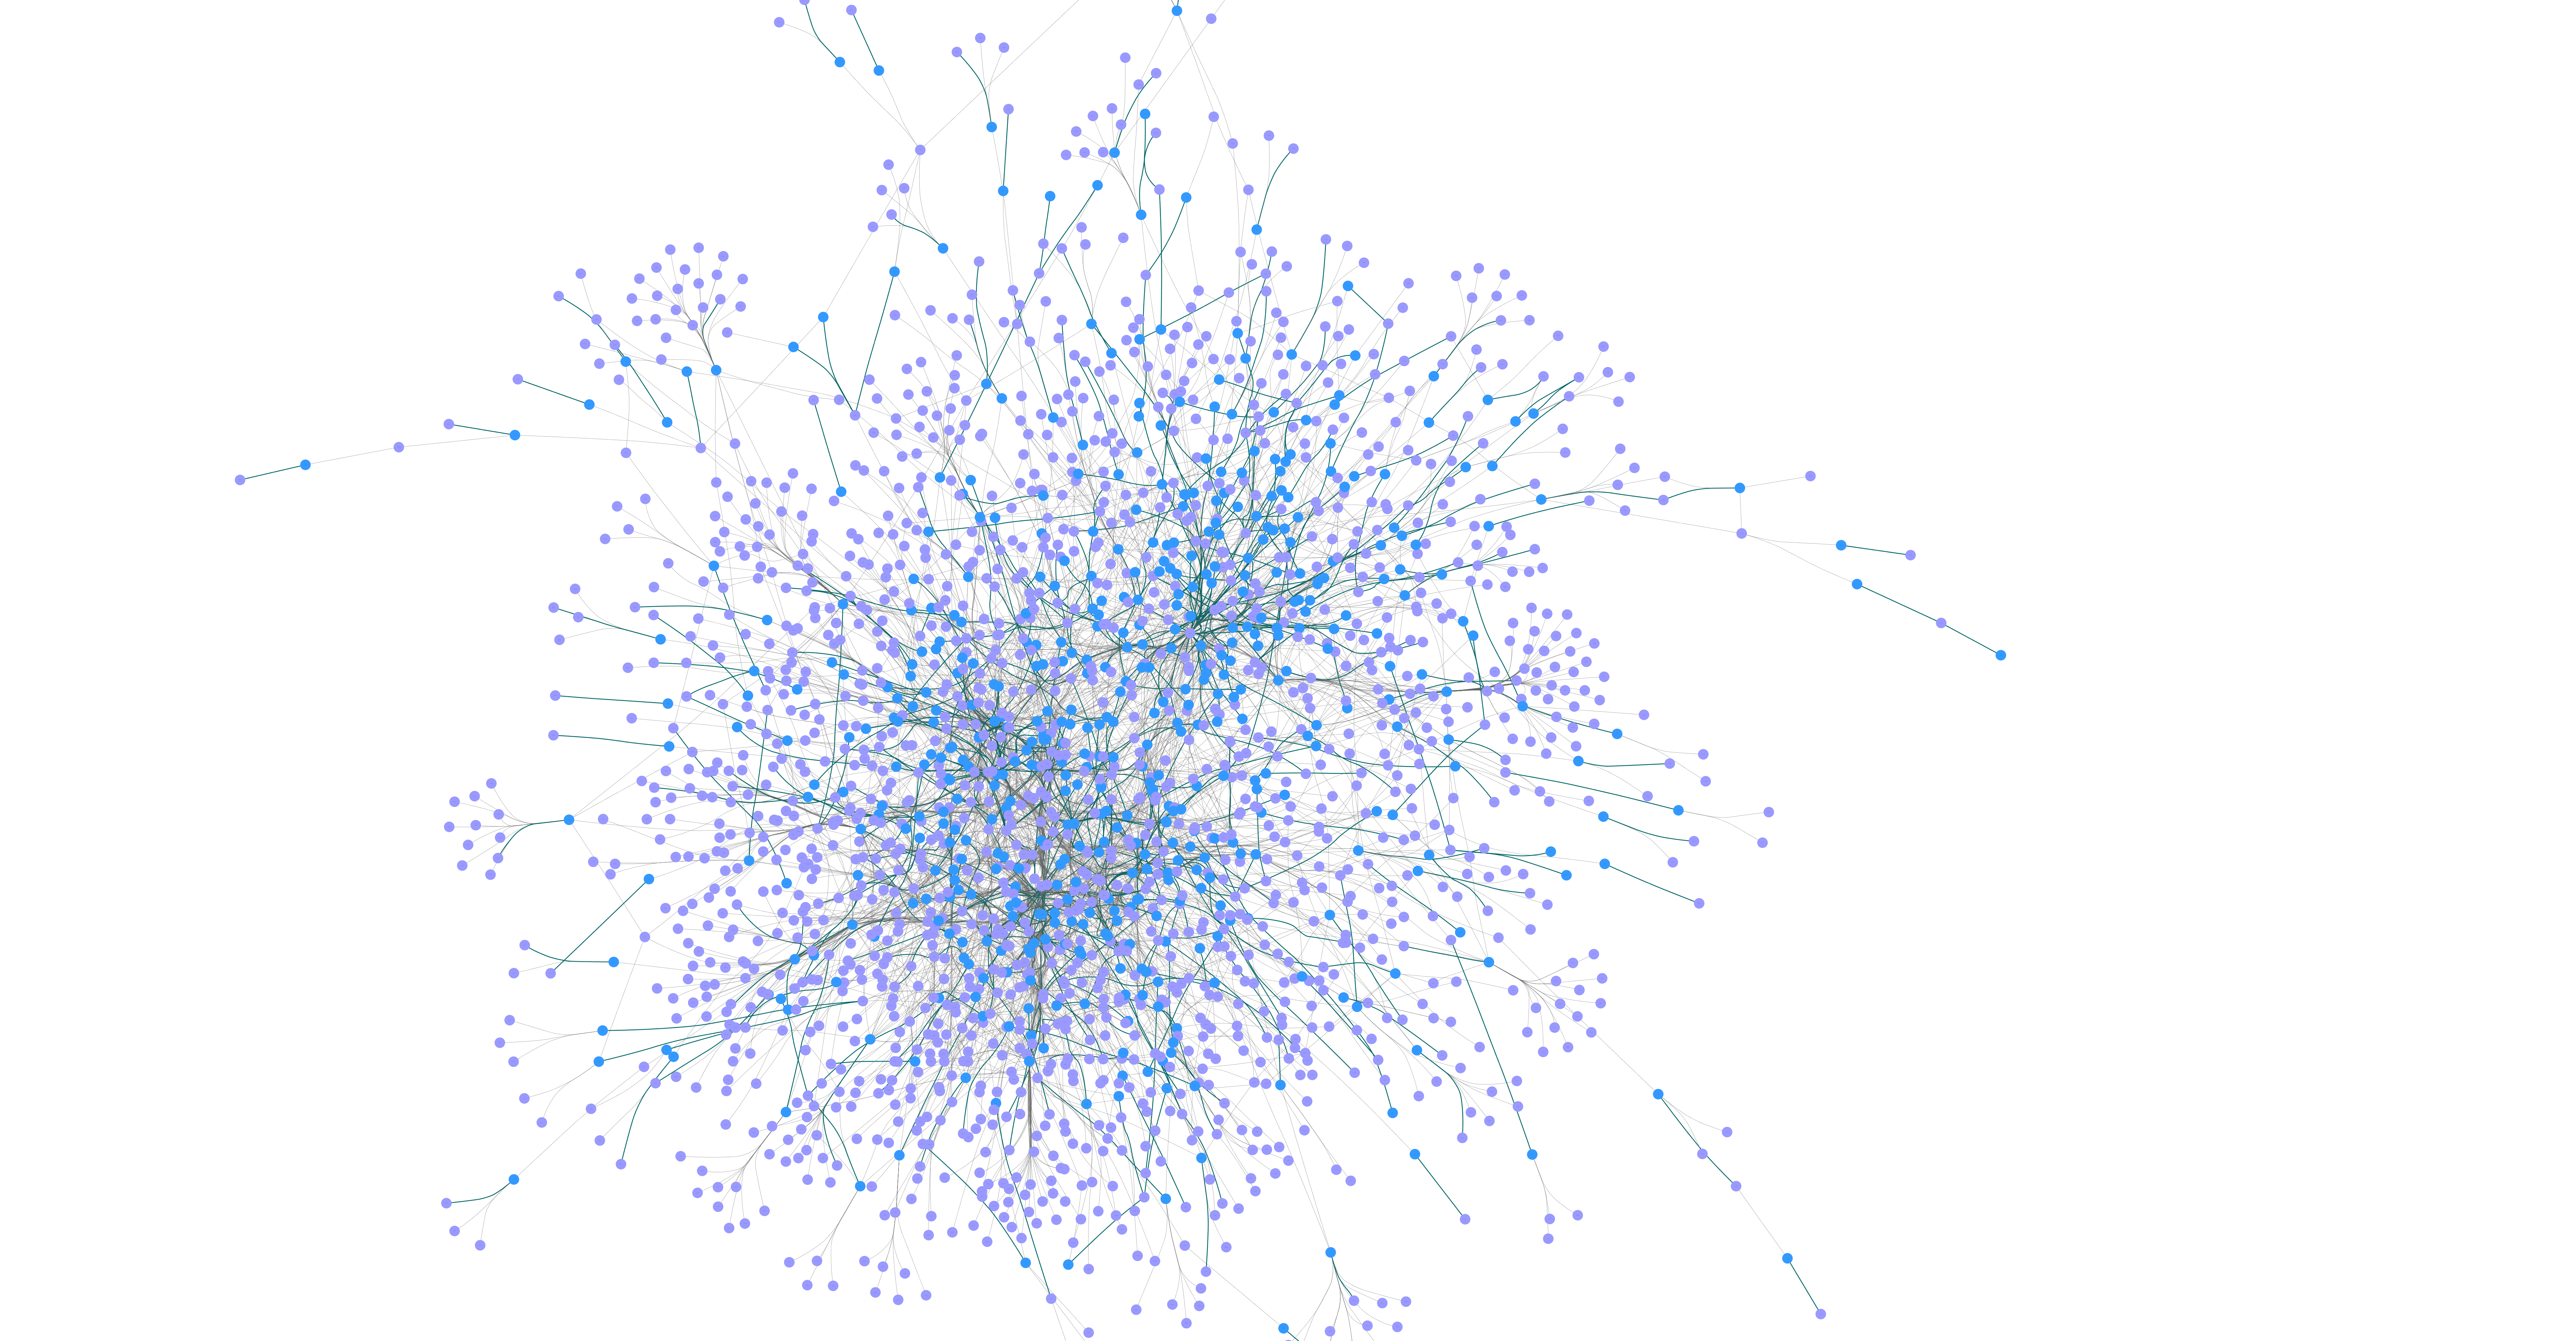
\includegraphics[width=0.5\textwidth]{Coraline_network.png}
    \caption{Network of Coraline fanfiction. Blue nodes represent stories, violet nodes represent users. Darker edges represent authorship, lighter edges represent a review.}
    \label{fig:my_label}
\end{figure}

\section{Conclusion}

\section{Appendix}

\subsection{Scraping FanFiction.Net}

The terms of service for FanFiction.Net state the limitations of launching automated bots in Section 4, Paragraph E of their terms of service\footnote{https://www.fanfiction.net/tos/}, paraphrased here:

\begin{itemize}
    \item ``You agree not to use or launch any automated system... that accesses the Website in a manner that sends more request messages... than a human can reasonably produce in the same period....''
    \item ``FanFiction.Net grants the operators of public search engines permission to use spiders... solely to the extent necessary for creating publicly available searchable indices... but not caches or archives....''
    \item ``You agree not to collect or harvest any personally identifiable information... for any commercial solicitation purposes.''
\end{itemize}

Scraping FanFiction.Net may be accomplished via the \texttt{scraper/} directory of this repository. The core documentation pertaining to each script and their respective functions are contained therein, this discussion pertains to the high-level idea of what they accomplish.

All users and stories on FanFiction.Net may be identified via a unique id-number. These id-numbers may be used to directly access one or the other, for example: user \textit{124}'s profile may be found by sending a request to https://www.fanfiction.net/u/124. In a similar manner, story \textit{124} would be at https://www.fanfiction.net/s/124. Reviews for a story follow the pattern \texttt{/r/125/0/1/}, where the first integer corresponds the story-id, the second integer to a certain chapter (or 0 for all reviews), and the third is a page number (a maximum of 15 reviews are displayed on each page, so any overflow will be on subsequent pages).

\bibliographystyle{aaai}
\bibliography{link-prediction-fanfiction}

\end{document}
